\documentclass{article}


\include{stddefs}
\include{imodefs}

\newcommand{\pd}[2]{\frac{\partial #1}{\partial #2}}

\begin{document}



\chapterno{7}
\chapter{Several variables}

A function of several variables usually refers to a function
\begin{equation}\label{semidef}
f: \RR^n \rightarrow \RR,
\end{equation}
where $n > 1$ is a natural number. We have already seen functions
of several variables with $n>1$. In particular, in Chapter \ref{whatisopt}, we
saw linear functions (in connection with linear programming) like
\begin{equation}\label{sv:linfunc}
f(x_1, x_2) = 3 x_1 + 2 x_2.
\end{equation}
This is a rather simple function of several variables with $n=2$ in \eqref{semidef}.
In general functions as in \eqref{semidef} can be wildly complicated. One of the main purposes
of this chapter is to zero in on the class of differentiable functions in \eqref{semidef}. In
Chapter \ref{chapter:convexfunctions} we defined what it means for a function of
one variable to be differentiable. This was inspired by a drawing of the graph of the
function. In several variables (for $n > 1$) one has to be a bit clever in the definition
of differentiability. The upshot is that the derivative at a point now is a row vector (or more generally a matrix)
instead of being a single number. As an example, using notation that we introduce in this chapter,
the derivative of the function in \eqref{sv:linfunc} at $(0, 0)$ is
$$
\left(\pd{f}{x_1}, \pd{f}{x_2}\right) = \left(3, 2\right).
$$
This notation means that partial differentiation with respect to a variable occurs i.e., one fixes
the variable and computes the derivative with respect to this variable viewing all the other variables as constants.

First some treasured memories from the author's past.


\section{Introduction}

Many years ago, I had a job as a financial analyst in a bank. This was long before a
financial analyst became a quant and machine learning became a buzz word. Digging through my
old notes from that time, I found the outlines below.

\includegraphics{nlpb.png}

These were notes I made in connection with modelling the yield curve
for zero coupon bonds.  I had to fit a very non-linear function in
\emph{several variables} to financial data and had to use effective
numerical tools (and \footnote{programming them}{\includegraphics{apl.png}} in 
\url{APL}{https://en.wikipedia.org/wiki/APL_(programming_language)}). Tools
that are also used today in machine learning and data science.

Ultimately we are interested in solving optimization problems like
  \begin{align*}
    &\text{Minimize} &f(x_1, \dots, x_n)\\
    &\text{with constraint}\\
    &&(x_1, \dots, x_n)\in C,
  \end{align*}
  where $C\subseteq \RR^n$ and $f:\RR^n\rightarrow \RR$ is a differentiable (read nice for now) function.

  Training neural networks is a fancy name for solving an optimization problem, where
  usually $C = \RR^n$ and $f$ is built just like in the least squares method from some
  data points. The difference is that in neural networks, $f$ is an incredibly complicated
  (differentiable) function composed of several intermediate functions. We do not, as in the method of
  least squares, have an explicit formula for finding a minimum. We have to
  rely on iterative methods. One such method is called \emph{gradient descent}.

  Let me illustrate this in the simplest case, where $n=1$. The general case is conceptually very similar
  (see Lemma \ref{gradientoptimization}).

  Suppose that
  $f$ is differentiable at $x_0$ with $f'(x_0)\neq 0$ and the we wish to
  solve the minimization problem
  \begin{align*}
    &\text{Minimize} &f(x)\\
    &\text{with constraint}\\
    &&x\in \RR.
  \end{align*}
  Solving the equation $f'(x) = 0$ (to find potential minima) may
  be difficult. Instead we try something else.
  
  We know for sure that $x_0$ is not a local minimum (why?). It turns out that we can
  move a little bit in the \footnote{direction}{Left if $f'(x_0) > 0$ and right if $f'(x_0) < 0$.} of $-f'(x_0)$  and get a better candidate for
  a minimum than $x_0$ i.e., for small $\lambda > 0$ and $h = -\lambda f'(x_0)$ we have
  $$
  f(x_0 + h) - f(x_0) < 0. 
  $$
  This is a \footnote{consequence}{If you use the definition of differentiability with $h = -\lambda f'(x_0)$, you will see that
    $$f(x_0 + h) - f(x_0) = - \lambda( f'(x_0)^2 + \epsilon(-\lambda f'(x_0)) f'(x_0)).$$ For small $\lambda > 0$ this shows that $f(x_0 + h) - f(x_0) < 0$, as $f'(x_0)^2 > 0$.} of the definition of $f$ being differentiable at $x_0$ with
  $f'(x_0)\neq 0$.

  
  The process is then repeated putting $x_0 := x_0 + h$ until the absolute value of $f'(x_0)$ is
  sufficiently small (indicating that we are close to a point $x$ with $f'(x) = 0$).


  As usual, the machine learning community has its own terms for
  rather established mathematical concepts:  they call the number $\lambda > 0$ 
  the \url{learning rate}{https://en.wikipedia.org/wiki/Learning_rate}.

  \beginshex
  Illustrate the gradient descent method for $f(x) = x^2$. Pay attention to
  the learning rate $\lambda > 0$. How big is $\lambda$ allowed to be, when
  $$
  f(x_0 + h) - f(x_0) < 0
  $$
  is required and $h = -\lambda f'(x_0)$?
  \endshex

  \beginshex
  This is a hands-on exercise: carry out the gradient descent method
  numerically for the function
  $$
  f(x) = (x-1)^4 + \sin(x)^2
  $$
  to solve the minimization problem
  \begin{align*}
    &\text{Minimize} &f(x)\\
    &\text{with constraint}\\
    &&x\in \RR
  \end{align*}
  starting with $x_0=1$.

  \begin{hideinbutton}{Hint}
    It is not clear how to choose the step size here. Proceed by letting $k$ be the
    smallest natural number, such that
    $$
    f(x_0 - 2^{-k} f'(x_0)) < f(x_0).
    $$
    Stop the process, when $|f'(x_0)| < 0.001$.
    
    \begin{hideinbutton}{Helpful code}
      \begin{sage}
def f(x):
  f = (x-1)^4 + sin(x)^2
  return f.n()

def fm(x):
  fm = 4*(x-1)^3 + 2*sin(x)*cos(x)
  return fm.n()

x0 = 1

print(f(x0))
for k in range(5):
  x1 = x0 - 2^(-k)*fm(x0)
  x2 = x1.n()
  print((k, x2, f(x2), fm(x2)))
\end{sage}
\end{hideinbutton}
\end{hideinbutton}

  
  Is $f$ a convex function?
  
  Explain how the \footnote{\url{Newton-Raphson method}{https://en.wikipedia.org/wiki/Newton\%27s_method}}{This is an iterative method for approximating a zero for a differentiable function $g(x)$. It works by guessing $x_0$ and then iterating $x_{i+1} = x_i - g(x_i)/g'(x_i)$ to get a sequence $x_0, x_1, \dots$ approximating a zero $z$ ($g(z) = 0$).} may be used to solve the minimization problem and
  compute the minimum also using this method.

  \begin{hideinbutton}{Helpful code}
\begin{sage}
def fm(x):
  fm = 4*(x-1)^3 + 2*sin(x)*cos(x)
  return fm.n()  

def fmm(x):
  fmm = 12*(x-1)^2 + 2*cos(x)^2 - 2*sin(x)^2
  return fmm.n()

def newtononestep(x0):
  newt = x0 - fm(x0)/fmm(x0)
  x1 = newt.n()
  return (x1, fm(x1))

newtononestep(1) 
\end{sage}      
  \end{hideinbutton}
  
  \begin{sage}
    plot((x-1)^4 + sin(x)^2, (x, 0, 1))
    \end{sage}
  \endshex
  
  Recall the definition of a function $f:\RR\rightarrow \RR$ being
differentiable at a point $x_0\in \RR$ with derivative $c = f'(x_0)$. Here we measured
the change $f(x_0+h) - f(x_0)$ of $f$ in terms of the change $h$ (in $x$). It had to have
the form
\begin{equation}\label{diffonedef}
f(x_0+h) - f(x_0) = c\, h + \epsilon(h) h,
\end{equation}
where $\epsilon:(-\delta, \delta)\rightarrow \RR$ is a function
continuous in $0$ with $\epsilon(0) = 0$ and $\delta>0$ small.
If you divide both sides of \eqref{diffonedef} by $h$ you recover
the usual more geometric definition of differentiability as
a limiting slope:
\begin{equation}\label{nondef}
\lim_{h\to 0}\, \frac{f(x_0 + h) - f(x_0)}{h} = c = f'(x_0).
\end{equation}

We wish to define differentiability at $x_0\in \RR^n$ for a function
$f: \RR^n\rightarrow \RR^m$. In this setting the quotient
$$
\frac{f(x_0 + h) - f(x_0)}{h} 
$$
in \eqref{nondef} does not make any sense. There is no way we can divide
a vector $f(x_0 + h) - f(x_0)\in \RR^m$ by a vector $h\in \RR^n$, unless
of course $m = n = 1$ as in \eqref{nondef}, where we faced
usual numbers.

The natural thing here is to generalize the definition in \eqref{diffonedef}.
First let us recall what functions $f:\RR^n\rightarrow \RR^m$ look like.



\section{Vector functions}

A function $f:\RR^n\rightarrow \RR^m$ takes a vector
$(x_1, \dots, x_n)\in \RR^n$ as input and gives a
vector $(y_1, \dots, y_m)\in \RR^m$ as output. This means
that every coordinate $y_1, \dots, y_m$ in the output
must be a function of $x_1, \dots, x_n$ i.e.,
$$
y_i = f_i(x_1, \dots, x_n)
$$
for $i = 1, \dots, m$. So in total, we may write $f$ as
\begin{equation}\label{sevformat}
f(x_1, \dots, x_n) =
\begin{pmatrix}
  f_1(x_1, \dots, x_n)\\
  \vdots \\
  f_m(x_1, \dots, x_n)
\end{pmatrix}.
\end{equation}

Each of the (coordinate) functions $f_i$ are functions from
$\RR^n$ to $\RR$.

\beginshex
Look back at Exercise \ref{perceptronex}. Write down precisely the
vector function $h:\RR^2\rightarrow \RR^2$ occuring there.
\endshex

\beginshex\label{rotate90ex}
The function $f:\RR^2\rightarrow \RR^2$ is rotating
a vector $90$ degress counter clockwise. What are
$f_1$ and $f_2$ in
$$
f(x, y) =
\begin{pmatrix}
  f_1(x, y)\\
  f_2(x, y)
\end{pmatrix}?
$$
\begin{hideinbutton}{Hint}
Try rotating some specific vectors like $(1, 0), (0, 1), (1, 1)$ $90$ degrees.
Do you see a pattern?
\end{hideinbutton}
\endshex

\section{Differentiability}

The definition of differentiability for a function
$f:\RR^n\rightarrow \RR^m$ mimics \eqref{diffonedef}, except
that $\epsilon(h) h$ is replaced by $\epsilon(h) |h|$. However,
in \eqref{diffonedef} one could just as easily, with the same
result, have replaced $\epsilon(h) h$ by $\epsilon(h) |h|$.

Notice, however, that now the derivate is a matrix!

\begin{definition}[emph]\label{diffdef}
Let $f:U\rightarrow \RR^m$ be a
  function with $U\subseteq \RR^n$ an open subset.  Then $f$ is
  \emph{differentiable} at $x_0\in U$ if there exists an $m\times n$
  matrix $C$, such that
  $$
    f(x_0 + h) - f(x_0) = C\, h + \epsilon(h)\, \abs{ h },
  $$
  where $\epsilon:O\rightarrow \RR^m$ is a function from an open
  subset $O\subseteq \RR^n$ containing $0$, such that $\epsilon$ is
  continuous in $0$ with $\epsilon(0) = 0$. In this case,
  the $m\times n$ matrix $C$ is called the (matrix) derivative of
  $f$ at $x_0$ and denoted by $f'(x_0)$.

  The function $f$ is called
  differentiable if it is differentiable at every $x\in U$.
\end{definition}

How do we compute the matrix derivative $C$ in the above definition?
We need to look at the representation of $f$ in \eqref{sevformat} and
introduce the partial derivatives.

\subsection{Partial derivatives}

\begin{definition}[emph]\label{partdif}
  Let $f: U\rightarrow \RR$ be a function, where $U$ is an open subset
  of $\RR^n$. Then we define the limit
  \begin{equation*}
    \frac{\partial f}{\partial x_i}(v): = \lim_{\delta\to 0} \,\frac{f(v +
      \delta e_i) - f(v)}{\delta},
  \end{equation*}
  for $i = 1, \dots, n$, where $e_i$ 
  is the \emph{$i$-th canonical basis vector} in $\RR^n$, $v\in U$ and
  $\delta\in \RR$. This limit is called the \emph{partial derivative}
  of $f$ with respect to $x_i$ at $v$.
\end{definition}

\begin{frameit}
\begin{remark}
Let us make Definition \ref{partdif} a bit more explicit:
The $i$-th canonical basis vector $e_i$ in $\mathbb{R}^n$ is the vector, which is $1$ at the $i$-th coordinate and $0$ elsewhere. Therefore 

$$
\begin{aligned}
&\dfrac{f(v + \delta e_i) - f(v)}{\delta} =\\ 
&\dfrac{f(x_1, \dots, x_i + \delta, \dots, x_n) - f(x_1, \dots, x_n)}{\delta},
\end{aligned}
$$

since

$$
v = \begin{pmatrix}x_1\\ \vdots\\ x_n \end{pmatrix}
$$

and

$$
v + \delta e_i = \begin{pmatrix}x_1\\ \vdots \\ x_i \\ \vdots \\ x_n \end{pmatrix} + \delta 
\begin{pmatrix} 0\\ \vdots\\ 1 \\ \vdots \\0 \end{pmatrix} = 
\begin{pmatrix}x_1\\ \vdots\\ x_i + \delta \\ \vdots \\ x_n \end{pmatrix}.
$$
\end{remark}
\end{frameit}

To get a feeling for the definition and computation of partial derivatives, take a look at the
example below.

\begin{example}\label{Examplepartdif}
  Consider the function $f: \RR^2 \rightarrow \RR$ given by
  \begin{equation*}
    f(x_1, x_2) = x_1 x_2^2 + x_1.
  \end{equation*}
  Then
  \begin{align*}
    \frac{\partial f}{\partial x_2}(v) &=
    \lim_{\delta\to 0}\frac{f(x_1, x_2 + \delta) - f(x_1, x_2)}{\delta}\\
    & = \lim_{\delta\to 0}
    \frac{x_1 (x_2+\delta)^2 + x_1 - (x_1 x_2^2 + x_1)}{\delta}\\
    &= x_1 \lim_{\delta\to 0}\frac{(x_2+\delta)^2 - x_2^2}{\delta} =
    x_1\, \lim_{\delta\to 0} (2 x_2 + \delta) = 2 x_1 x_2,
  \end{align*}
  where $v = (x_1, x_2)$. This example illustrates that
  $\frac{\partial f}{\partial x_i}$ can be computed just like in the
  one variable case, when the other variables ($\neq x_i$) are treated
  as constants. Notice that
  \begin{equation*}
    \frac{\partial}{\partial x_1}\frac{\partial f}{\partial x_2} =
    \frac{\partial }{\partial x_2}\frac{\partial f}{ \partial x_1} = 2
    x_2. 
  \end{equation*}

  
\end{example}

Partial derivatives behave almost like the usual derivatives of one
variable functions. You simply fix one variable that you
consider the "real" variable and treat the other variables as constants.

\begin{example}\label{exsagepd}
  $$
  \frac{\partial}{\partial x}\left( \sin(x y) + x^2 y^2 + y\right) = y \cos(x y) + 2 x y^2.
  $$
\end{example}

Below are examples of Sage code computing partial derivatives. Notice that the
variables must be declared first.

\begin{sage}
x1, x2 = var('x1, x2')
f = x1*x2^2 + x1
print(f.diff(x2)) # Compute partial derivative of f with respect to x2
print(f.diff(x2).diff(x1)) # Symmetry of partial derivatives
print(f.diff(x1).diff(x2)) # Symmetry of partial derivatives
\end{sage}

\beginshex
Use the Sage window above to verify the computation of the partial
derivative in Example \ref{exsagepd}.
\endshex

The following result tells us how to compute the matrix derivative.

\begin{proposition}[emph]\label{proppd}
  Let $f:U\rightarrow \RR^m$ be a function with $U\subseteq \RR^n$ an
  open subset. If $f$ is differentiable at $x_0\in U$, then the
  partial derivatives
  \begin{equation*}
    \frac{\partial f_i}{\partial x_j}(x_0)
  \end{equation*}
  exist for $i = 1, \dots, m$ and $j = 1, \dots, n$ and the matrix $C$
  in Definition \ref{diffdef} is
  \begin{equation*}
    C =
    \begin{pmatrix}
      \dfrac{\partial f_1}{\partial x_1}(x_0) & \cdots &
      \dfrac{\partial f_1}{\partial x_n}(x_0)\\
      \vdots & \ddots & \vdots \\
      \dfrac{\partial f_m}{\partial x_1}(x_0) & \cdots &
      \dfrac{\partial f_m}{\partial x_n}(x_0)
    \end{pmatrix}.
  \end{equation*}
\end{proposition}
  \begin{proof}[showhide]
    The $j$-th column in $C$ is $C e_j$. Putting $h = \delta e_j$ for
  $\delta\in \RR$ in Definition \ref{diffdef} gives
  \begin{equation*}
    f(x_0 + \delta e_j) - f(x_0) = \delta C e_j + \epsilon(\delta e_j)
    \abs{ \delta }.
  \end{equation*}
  The $i$-th coordinate of this identity of $m$-dimensional vectors
  can be written
  \begin{equation}\label{pdshow1}
    f_i(x_0 + \delta e_j) - f_i(x_0) = \delta C_{i j} + \tilde{\epsilon}_i(\delta)
    \delta
  \end{equation}
  where
  \begin{equation*}
    \tilde{\epsilon}_i(\delta) = 
    \begin{cases}
      \epsilon_i(\delta e_j) \dfrac{\abs{ \delta }}{\delta} &\text{if } \delta\neq 0 \\
      0 &\text{if } \delta = 0
    \end{cases}
  \end{equation*}
  and \eqref{pdshow1} shows that $C_{ij} = \frac{\partial f_i}{\partial x_j}(x_0)$.
    \end{proof}

\beginshex
Compute the matrix derivative of the vector function in Exercise \ref{rotate90ex}.
\endshex

For a function $f:U\rightarrow \RR$ with $U\subseteq \RR^n$
an open subset, the partial derivative, if it exists for every $x\in
U$, is a new function
\begin{equation*}
  \frac{\partial f}{\partial x_j} : U\rightarrow \RR.
\end{equation*}
We will use the notation
\begin{equation*}
  \frac{\partial^2 f}{\partial x_i \partial x_j}
  :=\frac{\partial}{\partial x_i} \frac{\partial f}{\partial x_j}
\end{equation*}
for the \emph{iterated (second order) partial derivative}.

The first part of following result is a converse to
Proposition \ref{proppd}. The second part contains the surprising
\emph{symmetry of the second order partial derivatives} under rather mild
conditions. We will not go into the proof.

\begin{theorem}[emph]\label{partsymm}
  Let $f:U\rightarrow \RR^m$ be a function with $U\subseteq \RR^n$ an
  open subset. If the partial derivatives for $f$ exist at every $x\in U$ with
  \begin{equation*}
    \frac{\partial f_i}{\partial x_j}
  \end{equation*} 
  continuous (for $i = 1, \dots, m$ and $j = 1, \dots, n$), then $f$
  is differentiable. If the second order partial
  derivatives exist for a function 
 $f : U\rightarrow \RR$ and are continuous functions,
  then
  \begin{equation*}
    \frac{\partial^2 f}{\partial x_i \partial x_j} = \frac{\partial^2
      f}{\partial x_j \partial x_i}
  \end{equation*}
  for $i, j = 1, \dots, n$.
\end{theorem}

\beginshex
Verify (by hand!) the symmetry of the second order partial derivatives for the function
$f$ in Example \ref{exsagepd} i.e., show that
  \begin{equation*}
    \frac{\partial^2 f}{\partial x \partial y} = \frac{\partial^2
      f}{\partial y \partial x}.
  \end{equation*}
\endshex

\beginshex
Verify that $f: \RR^2\rightarrow \RR$ given by
$$
f(x, y) = \frac{x^2 y}{1 + y^2}
$$
is a differentiable function by computing
$$
\frac{\partial f}{\partial x}\qquad\text{and}\qquad\frac{\partial f}{\partial y}
$$
and applying Theorem \ref{partsymm}. Check also that
  \begin{equation*}
    \frac{\partial^2 f}{\partial x \partial y} = \frac{\partial^2
      f}{\partial y \partial x}.
  \end{equation*}
\endshex

\section{Newton-Raphson in several variables!}


There is a beautiful generalization of the Newton-Raphson method to several variable
functions $f:\RR^n\rightarrow \RR^n$. Consider first that you would
like to solve the system
\begin{align}\label{newtsevex}
  y^2-x^3 + x &= 0\\
  y^3-x^2 &= 0
\end{align}
of non-linear equations in the two variables $x$ and $y$. Notice that
we are talking \emph{non-linear} here. This is so much more
difficult than the systems of linear equations that you
encountered in a previous chapter.

However, just like we used Newton's method in one variable for solving
a non-linear equation, Newton's method for finding
a zero for a function $f: \RR^n\rightarrow \RR^n$ generalized to the
iterative scheme
\begin{frameit}
\begin{equation}\label{onestepmultnewt}
  x_{i+1} = x_i - f'(x_i)^{-1} f(x_i)
\end{equation}
\end{frameit}
provided that the $n\times n$ matrix derivative $f'(x_i)$ is invertible.

The reason that \eqref{onestepmultnewt} works comes again from the
powerful definition of differentiability in Definition \ref{diffdef} using that
  \begin{equation}\label{eqdiffnewt}
  f(x) - f(x_0)\qquad \text{is close to}\qquad f'(x_0) (x - x_0)
\end{equation}
provided that $h = x - x_0$ is small. In fact, you get (again)
\eqref{onestepmultnewt} from \eqref{eqdiffnewt} by putting $f(x)$ to
$0$, replacing \emph{is close to} by $=$ and then isolating $x$.

For the equations in \eqref{newtsevex}, the iteration scheme \eqref{onestepmultnewt} becomes

\begin{equation}\label{exnewtmult}
    \begin{pmatrix}
      x_{i+1} \\ y_{i+1}
    \end{pmatrix} =
    \begin{pmatrix}
      x_i\\ y_i
    \end{pmatrix} -
    \begin{pmatrix}
      - 3 x_i^2+1 & 2 y_i\\
      -2 x_i & 3 y_i^2
    \end{pmatrix}^{-1}
    \begin{pmatrix}
      y_i^2-x_i^3 + x_i\\ y_i^3 - x_i^2
    \end{pmatrix}.
  \end{equation}

  \beginshex
  Verify the claim in \eqref{exnewtmult} by applying \eqref{onestepmultnewt} to
  $$
  f(x, y) =
  \begin{pmatrix}
    y^2 - x^3 + x\\
    y^3 - x^2
  \end{pmatrix}.
  $$
  Carry out sufficiently many iterations starting with the vector $(1, 1)$ in
  \eqref{exnewtmult} to see the iteration stabilize. You should do this
  using a computer.
  \endshex


  
  \section{Local extrema in several variables}

For a function
$f:U\rightarrow \RR$, where $U\subseteq \RR^n$, the derivative
$f'(v)$ at $v\in U$ is called \emph{the gradient}
for $f$ at $v$. Classically, it is denoted $ \nabla f(v)$ i.e.,
$$
\nabla f(v) = \left(\frac{\partial f}{\partial x_1}(v), \dots, \frac{\partial f}{\partial x_n} (v)\right).
$$
The definition below is stolen from the one variable case.

\begin{definition}[emph]\label{Critptsevvar}
  Let $f:U\rightarrow \RR$ be a function, where $U\subseteq \RR^n$ is
  an open subset. Suppose that the partial derivatives exist at
  $x_0\in U$. Then $x_0$ is called a \emph{critical
    point} for $f$ if $\nabla f(x_0)=0$.
\end{definition}

  \begin{example}
    Consider the function $f: \RR^2 \rightarrow \RR^2$ given by
    $$
    f\begin{pmatrix} x \\ y \end{pmatrix} =
    \begin{pmatrix}
      2 x + 3 \log(y)\\
      3 x / y - 3 y^2
      \end{pmatrix}
      $$
      corresponding to finding critical points for the function
      \begin{equation}\label{newsurf}
      g(x, y) = x^2 + 3 x \log(y) - y^3.
      \end{equation}
        
  You can left click and hold the graph computed below (after it has rendered) and rotate
  the surface to get a feeling for what \eqref{newsurf} looks like. Zooming in is also possible.
  
\begin{sage}
x, y = var('x, y')
plot3d(x^2 + 3*x*log(y) - y^3, (x, 0.25, 1), (y, 0.5, 1), 
adaptive=True, color=rainbow(60, 'rgbtuple'))
\end{sage}


      
      Here
      $$
      f' =
      \begin{pmatrix}
        2 & 3/y \\
        3/y & -3 x/y^2 - 6 y
      \end{pmatrix}.
      $$

      In the Sage code below, Newton's method is started at $(1, 1)$ and iterated four times.
      
      \begin{sage}
import numpy as np
import numpy.linalg as la

def f(x):
  return np.array([2*x[0] + 3*log(x[1]), 3*x[0]/x[1] - 3*x[1]*x[1]])

def df(x):
  return np.array([[2, 3/x[1]], [3/x[1], -3*x[0]/x[1]^2 - 6*x[1]]]) 

def newton(x):
   s = la.solve(df(x), f(x)) # Corresponds to f'(x)^{-1} f(x).  
   return x - s

v0 = np.array([1, 1])

v1 = newton(v0)
print(v1)
v2 = newton(v1)
print(v2)
v3 = newton(v2)
print(v3)
v4 = newton(v3)
print(v4)
\end{sage}
\end{example}




If $x_0$ is not a critical point for $f$ we can use the gradient
vector to move in a direction making $f$ strictly smaller/larger. This is
very important for optimization problems.



\begin{lemma}[emph]\label{gradientoptimization}
  Let $f: U\rightarrow \RR$ be a differentiable function, where
  $U\subseteq \RR^n$ is an open subset. Suppose that $u\in \RR^n$ and
  $\nabla f(x_0) u < 0$ for $x_0\in U$. Then
  \begin{equation*}
    f(x_0 + \lambda u) < f(x_0)
  \end{equation*}
  for $\lambda > 0$ small.
\end{lemma}
\begin{proof}[showhide]
  By the differentiability of $f$,
  \begin{equation*}
    f(x_0 + u) - f(x_0) = \nabla f(x_0) u + \epsilon(u) |u|,
  \end{equation*}
  where $\epsilon:\RR^n \rightarrow \RR$ is a function satisfying
  $\epsilon(h) \rightarrow 0$ for $h\rightarrow 0$. For $\lambda > 0$
  with $x_0 + \lambda u\in U$ we have
  \begin{equation*}
    f(x_0 + \lambda u) - f(x_0) = \lambda (\nabla f(x_0) u +
    \epsilon(\lambda u) 
    | u |).
  \end{equation*}
  When $\lambda$ tends to zero from the right, it follows that $f(x_0 + \lambda u) - f(x_0) <
  0$ for small $\lambda > 0$.
\end{proof}


The result below is the multi variable generalization of looking for
local extrema by putting $f'=0$ in the one variable case.

\begin{proposition}[emph]\label{locopt}
  Let $f: U\rightarrow \RR$ be a differentiable function, where
  $U\subseteq \RR^n$ is an open subset. If $x_0\in U$ is a local
  extremum, then $x_0$ is a critical point for $f$.
\end{proposition}
\begin{proof}[showhide]
  Suppose that $\nabla f(x_0)\neq 0$.  If $x_0$ is a local minimum,
  then we may use $u = -\nabla f(x_0)$ in
  Lemma \ref{gradientoptimization} to deduce that $f(x_0 + \lambda u) <
  f(x_0)$ for $\lambda>0$ small. This contradicts the local minimality
  of $x_0$.  If $x_0$ is a local maximum we can apply
  Lemma \ref{gradientoptimization} with $-f$ and $u = \nabla f(x_0)$
  to reach a similar contradiction.  Therefore $\nabla f(x_0)=0$ and
  $x_0$ is a critical point for~$f$.
\end{proof}



\beginshex\label{exsaddlept}
Compute the critical points of
$$
f(x, y) = x^3 + x y + y^3.
$$
Is $(0,0)$ a local maximum or a local minimum for $f$?

\begin{hideinbutton}{Hint}
Look at 
\begin{align*}
f_1(t) &= f(t, t)\\
f_2(t) &= f(t, -t)
\end{align*}
and $f_1''(0)$ and $f_2''(0)$ (along with Theorem \ref{derconv}).
\end{hideinbutton}
\endshex

\beginshex
We will prove later that a differentiable function $f:\RR^2\rightarrow \RR$ is
strictly convex if the socalled Hessian matrix given by
$$
\begin{pmatrix}
  \dfrac{\partial^2 f}{\partial x^2}(v) &   \dfrac{\partial^2 f}{\partial x \partial y}(v) \\[1em]
  \dfrac{\partial^2 f}{\partial y \partial x}(v) &   \dfrac{\partial^2 f}{\partial y^2}(v)
\end{pmatrix}
$$
is positive definite for every $v\in \RR^2$. This is a multivariable generalization of
the fact that $g: \RR\rightarrow \RR$ is strictly convex if $g''(x) > 0$ for every
$x\in \RR$.

Now let
\begin{equation}\label{deffc}
f(x, y) = x^2 + y^2 - \cos(x) -\sin(y).
\end{equation}

\begin{hideinbutton}{3D graph}
  You can left click the surface computed below after it has rendered and  rotate
  or zoom in.
\begin{sage}
x, y = var('x, y')
plot3d(x^2 + y^2 - cos(x) -sin(y), (x, -1, 1), (y, -1, 1), adaptive=True, color=rainbow(60, 'rgbtuple'))
\end{sage}
\end{hideinbutton}

\begin{enumerate}[(a)]
\item
  Show that $f$ is strictly convex.
\item
  Compute the critical point(s) of $f$.
\item
  For a differentiable convex function $f:\RR^2\rightarrow \RR$ we have in general that
  \begin{equation}\label{nabla722}
  f(v) \geq f(u) + \nabla f(u) (v-u)
  \end{equation}
  for every $u, v\in \RR^2$. This is a multivariable generalization of Theorem \ref{fp}.

  Explain how one can use \eqref{nabla722} to compute a global minimum for the function $f$ in \eqref{deffc}. Is this minimum unique? Is
  $f(x, y)\geq -1$ for every $x, y\in \RR$?
\end{enumerate}
  \endshex

\section{The chain rule}

Recall the chain rule for functions of one variable. Here we have
functions $f:(a, b)\rightarrow \RR$ and $g:(c, d)\rightarrow \RR$,
such that $g(x)\in (a, b)$ for $x\in (c, d)$. If $g$ is differentiable at $x_0\in (c, d)$ and $f$
 is
differentiable at $g(x_0)\in (a, b)$, the chain rule says that $f\circ
g$ is differentiable at $x_0$ with
\begin{equation*}
  (f\circ g)'(x_0) = f'(g(x_0)) g'(x_0).
\end{equation*}
This rule generalizes verbatim to functions of several variables:
\begin{equation*}
  (f\circ g)'(x_0) = f'( g(x_0)) g'(x_0)
\end{equation*}
for compatible multivariate functions $f$ and $g$ when you replace
usual multiplication by matrix multiplication. 

\begin{theorem}[emph]\label{chainrule}
  Let $f:U\rightarrow \RR^m$ and $g: V\rightarrow \RR^n$ with
  $U\subseteq \RR^n$, $V\subseteq \RR^l$ open subsets and
  $g(V)\subseteq U$. If $g$ is differentiable at $x_0\in V$ and $f$ is
  differentiable at $g(x_0)\in U$, then $f\circ g$ is differentiable
  at $x_0$ with
  \begin{equation*}
    (f\circ g)'(x_0) = f'( g(x_0)) g'(x_0).
  \end{equation*}
\end{theorem}

The proof of the chain rule in this general setting uses
Definition \ref{diffdef} just as in the one variable
case. It is not conceptually difficult, but severely
cumbersome. We will not give it here.


\begin{example}
Consider $f:\RR^2\rightarrow \RR$ given by 
$$
f(x, y) = x^2 + y^2
$$ 
and
$g:\RR \rightarrow \RR^2$ given by
$$
g(t) = \begin{pmatrix}
t^2\\
t^3
\end{pmatrix}.
$$
We wish to use the chain rule to compute $(f\circ g)'(t)$. Now,
$f'(v)$ is a $1\times 2$ matrix and $g'(t)$ is a $2\times 1$ matrix
and the chain rule reads
\begin{align*}
(f\circ g)'(t) &= f'(g(t)) g'(t) \\
&= \begin{pmatrix} \pd{f}{x}(t^2, t^3) & \pd{f}{y}(t^2, t^3) \end{pmatrix}
\begin{pmatrix}
2 t\\
3 t^2
\end{pmatrix} =\\
&= \pd{f}{x}(t^2, t^3) 2 t + \pd{f}{y}(t^2, t^3) 3 t^2 \\
&= 4 t^3 + 6 t^5.
\end{align*}
Of course, this agrees with the computation
$$
(f\circ g)(t) = t^4 + t^6.
$$
But, often you cannot hope to be able to compute the function and then find
the derivative. Here the chain rule may come in handy (as in backpropagation in
training neural networks).
\end{example}


\subsection{Computational graphs and the chain rule}

Consider a composition of the functions $f:\RR^m\rightarrow \RR^n$ and
$C: \RR^n\rightarrow \RR$. This gives a composite function
$$
F = C\circ f: \RR^m\rightarrow \RR.
$$
The chain rule then says that
$$
F'(x) = C'(u) F'(x)
$$ for
a vector $x\in \RR^m$ and $u = f(x)$. Notice that this is a matrix
product between a $1\times n$ matrix and an $n\times m$ matrix.


Let us write it out. Suppose that 
$$
f(x) = 
f
\begin{pmatrix}
  x_1\\ \vdots \\ x_m
\end{pmatrix} =
\begin{pmatrix}
  u_1(x_1, \dots, x_m) \\ \vdots \\ u_m(x_1, \dots, x_m)
\end{pmatrix}
$$

and
$$
C(u) = C
\begin{pmatrix} u_1\\ \vdots \\ u_n
\end{pmatrix}.
$$
Then
$$
\frac{\partial F}{\partial x_i} =
\frac{\partial C}{\partial u_1}\frac{\partial u_1}{\partial x_i} + \cdots +
\frac{\partial C}{\partial u_m} \frac{\partial u_m}{\partial x_i}
$$
for $i = 1, \dots, m$.


This is simply writing out the matrix multiplication
$$
  C'(u) f'(x) =
  \begin{pmatrix}
    \frac{\partial C}{\partial u_1} & \cdots & \frac{\partial C}{\partial u_m}
  \end{pmatrix}
  \begin{pmatrix}
    \frac{\partial u_1}{\partial x_1} & \cdots & \frac{\partial u_1}{\partial x_n}\\
    \vdots & \ddots & \vdots \\
   \frac{\partial u_m}{\partial x_1} & \cdots & \frac{\partial u_m}{\partial x_n}
  \end{pmatrix}.
$$

\begin{example}
  Consider three innocent functions $f, g, C: \RR\rightarrow \RR$ given by
  \begin{align*}
    f(x) &= \alpha x + \beta\\
    g(x) &= \gamma x + \delta\\
    C(x) &= x^2,
  \end{align*}
  where $\alpha, \beta, \gamma, \delta\in \RR$.
  Then the composite $F = C\circ g\circ f$ is also a function $\RR\rightarrow
  \RR$. Let us turn things upside down. If we fix $x\in \RR$ and let
  $\alpha, \beta, \gamma\, \delta\in \RR$ vary, then $F$ may be viewed
  as a function $\RR^4\rightarrow \RR$. Here $C'(u) = 2 u$ and
  $$
  F'(w) = \begin{pmatrix}
    \frac{\partial F}{\partial \alpha} &
    \frac{\partial F}{\partial \beta} &
    \frac{\partial F}{\partial \gamma} &
    \frac{\partial F}{\partial \delta} 
  \end{pmatrix} =
  C'(u) u'(w) = 2 u u'(w),
  $$
  where
  $$
  u = u(\alpha, \beta, \gamma, \delta) = (g\circ f)(\alpha, \beta, \gamma, \delta) = \gamma ( \alpha x + \beta) + \delta.
  $$

\end{example}

\begin{example}
  
It is often complicated to apply the chain rule if the
function $f:\RR^n\rightarrow \RR^m$ is composed of many
functions. To organize the computation of $f'(x_0)$ one
works with the socalled \emph{computational graph} of $f$.

A computational graph is made up of several nodes and directed edges.



We will consider the example
$$
f(x, y) =   \sin(x y) + x^2 y^2 + y
$$
from Example \ref{exsagepd}. Even though $f(x, y)$ superficially looks rather simple,
it is composed of several smaller functions as displayed in the computational graph

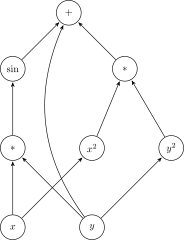
\includegraphics{fsevgraph.svg}

Every node in the above graph, except the input nodes (with no ingoing arrows),
represent some function $f:\RR^n\rightarrow \RR^m$. For example the node
$\sin$ represents a function $f: \RR\rightarrow \RR$ and $*$ represents
a function $f: \RR^2\rightarrow \RR$.

To emphasize that the non-input nodes really are functions we replace them by letters:

\includegraphics{fsevgraphfunct.svg}

Here we see that 
$$
f(x, y) = F(a(c(x, y)), y, b(d(x), e(y))), 
$$
where
\begin{align*}
  F(a, y, b) &= a + y + b\\
  a(c) &= \sin(c)\\
  c(x, y) &= x y\\
  b(d, e) &= d e\\
  d(x) &= x^2\\
  e(y) &= y^2
\end{align*}


The gradient is then available from the decorated graph below

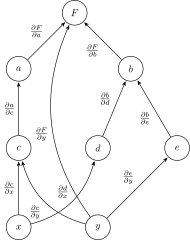
\includegraphics{fsevgraphfunctpd.svg}

by multiplying the decorations on each path from the top to the input variable and the summing up. For example,
$$
\pd{F}{x} = \pd{F}{a} \pd{a}{c} \pd{c}{x} + \pd{F}{b} \pd{b}{d} \pd{d}{x}.
$$

  Unfortunately the Sage plugin does not support \texttt{tensorflow}, but if you have a
  Google (gmail) account you can experiment with \texttt{tensorflow} (on GPUs and TPUs!) using \url{https://colab.research.google.com}{https://colab.research.google.com}. Below is an example for you to try out. It is related to the computational graph above.
  \begin{code}
import tensorflow as tf

x = tf.Variable(1.0)
y = tf.Variable(1.0)

with tf.GradientTape() as comp:
   c = x*y
   d = x**2
   e = y**2
   b = d*e
   a = tf.sin(c)
   F = a + b + y

derx = comp.gradient(F, x)
print(derx)   
\end{code}
\end{example}

\beginshex
Construct a computational graph for
$$
f(x, y) = x^3 + x y + y^3
$$
and detail the computation of the gradient $\nabla f$ in this context.

\begin{hideinbutton}{Tensorflow experiment (extra)}

  Compute the
gradient of $f$ for $(x, y) = (1, 1)$ using \texttt{tensorflow} on \url{https://colab.research.google.com}{https://colab.research.google.com}.
\end{hideinbutton}
\endshex




\beginshex
Consider $f: \RR\rightarrow \RR^3$ and $g:\RR^3\rightarrow \RR$
  given by
  \begin{equation*}
    f(t) =
     \begin{pmatrix}
       t\\ t^2\\ t^3
     \end{pmatrix}\qquad \text{and}\qquad g
    \begin{pmatrix}
       x\\ y\\ z
     \end{pmatrix} = x^2 + 3 y^6 + 2 z^5.
  \end{equation*}
  Compute $(g\circ f)'(t)$ using the chain rule and check the result
  with an explicit computation of the derivative of $g\circ f:
  \RR\rightarrow \RR$.
\endshex


\beginshex
We wish to show that the function $f: \RR^2 \rightarrow \RR$ given by
$$
f(x, y) = x^2 + y^2
$$
is convex. This means that we need to prove that
$$
f((1-t)x_0 + t x_1, (1-t) y_0 + t y_1) \leq (1-t) f(x_0, y_0) + t f(x_1, y_1)
$$
for every $(x_0. y_0), (x_1, y_1)\in \RR^2$ and every $t$ with $0\leq t\leq 1$.
This can be accomplished from the one variable case in the following way. Define
$$
g(t) = f((1-t)x_0 + t x_1, (1-t) y_0 + t y_1)
$$
and show that $g$ is convex by using the chain rule to show that $g''(t) \geq 0$. Show
how the convexity of $f$ follows from this by using that
$$
g(t) = g((1-t)\cdot 0 + t\cdot 1).
$$
\endshex

\section{Logistic regression}

The beauty of the sigmoid function is that it takes any value $x\in \RR$ and turns it into
a probability $0< \sigma(x) < 1$ by
$$
\sigma(x) =  \frac{1}{1 + e^{-x}},
$$
i.e., $\sigma(-\infty) = 0$ and $\sigma(\infty) = 1$.

\begin{hideinbutton}{Graph of the sigmoid function}
  \begin{sage}
    plot(1/(1 + exp(-x)), (x, -10, 10))
  \end{sage}
\end{hideinbutton}


\beginshex
Prove that
$$
\sigma'(x) =  \sigma(x) (1-\sigma(x))
$$
and
$$
\log \frac{\sigma(x)}{1-\sigma(x)} = x.
$$
\endshex

We will not go into all the details (some of which can be traced
to your course in introductory probability and statistics), but
suppose that we have an outcome $E$, which may or may not happen.

We have an idea, that the probability of $E$ is
dependent on certain parameters $w_0, w_1, \dots, w_n$ and
observations $x_1, \dots, x_n$ that fit into the sigmoid function as
\begin{equation}\label{probdist}
p(x_1, \dots, x_n) = \sigma(w_0 + w_1 x_1 + \cdots + w_n x_n) = \frac{1}{1 + e^{-w_0 - w_1 x_1 - \cdots - w_n x_n}}.
\end{equation}

An example of this could be where $x_1, \dots, x_{784}$ denote the
gray scale of each pixel in a $28\times 28$ image. The event $E$
is whether the image contains the digit $4$:

\includegraphics{four.png}

Here $p(x_1, \dots, x_{784})$ would be the probability that the image contains the digit $4$.

\subsection{Estimating the parameters}

Suppose also that we have a table of observations (data set)

\begin{equation}\label{mnist}
\begin{matrix}
  x_{11} & \cdots & x_{1n} & E_1\\
  x_{21} & \cdots & x_{2n} & E_2\\
  \vdots & \ddots & \vdots & \vdots\\
  x_{m1} & \cdots & x_{mn} & E_m,
\end{matrix}
\end{equation}

where each row has observations $x_{i1}, \dots, x_{in}$ along with a
binary variable $E_i$, which is $1$ if $E$ was observed to occur and
$0$ if not.

Assuming that \eqref{probdist} holds, the probability of observing the
$m$ observations in \eqref{mnist} is
\begin{equation}\label{lh}
\prod_{i=1}^m p(x_{i1}, \dots, x_{in})^{E_i} (1 - p(x_{i1}, \dots, x_{in}))^{1-E_i}.
\end{equation}
Notice that \eqref{lh} is a function $L(w_0, \dots, w_n)$ of the
parameters $w_0, w_1, \dots, w_n$ for fixed observations $x_1,\dots, x_n$.

We wish to choose the parameters so that $L(w_0, w_1, \dots, w_n)$ is
maximized (this is called \url{maximum likelihood
  estimation}{https://en.wikipedia.org/wiki/Maximum_likelihood_estimation}).
So we are in fact here, dealing with an optimization problem, which is
usually solved by gradient descent (for $-L$) or solving the equations
$$
\nabla L (w_0, w_1, \dots, w_n) = 0.
$$
 
Instead of maximizing $L(w_0, \dots, w_n)$ one usually maximizes the logarithm
\begin{align*}
\ell(w_0, w_1, \dots, w_n) &= \log L(w_0, w_1, \dots, w_n)\\
                           &= \sum_{i=1}^m E_i \log p(x_{i1}, \dots, x_{in}) + (1 - E_i) \log ( 1 - p(x_{i1}, \dots, x_{in}))\\
  &= \sum_{i=1}^m E_i (w_0 + w_1 x_{i1} + \cdots + w_n x_{in}) -  \log (1 + e^{w_0 + w_1 x_{i1} + \cdots + w_n x_{in}}).
\end{align*}



\begin{example}\label{exlogist}
  Suppose that the event $E$ is assumed to be dependent on only one observation $x$ i.e., $n=1$ above.
  For example, $E$ could be the event of not showing up on a Monday paired with the amount of sleep
  $x$ in the weekend.
  
  Here
  $$
  p(x) = \sigma(\alpha + \beta x)
  $$
  and
  \begin{align*}
  \ell(\alpha, \beta) &= \sum_{i=1}^m E_i \log p(x_i) +
                        (1 - E_i)\log (1-p(x_i))\\
                      &= \sum_{i=1}^m E_i (\alpha + \beta x_i) - \log(1 + e^{\alpha + \beta x_i}).
  \end{align*}
\end{example}


\beginshex

Explain how the end result of the computation of $\ell(\alpha, \beta)$ in Example \ref{exlogist} is obtained and
compute $\nabla \ell (\alpha, \beta)$.
\endshex


\begin{example}\label{challengerexample}
  I remember exactly where I was when first hearing about
  the Challenger disaster in 1986.

      \youtube{fSTrmJtHLFU}

  This dreadful event was caused by failure of a socalled O-ring. The
  O-rings had been tested before the launch for failure (=1 below) at different
  temperatures (in F) resulting in the (partial) table below.
  $$
  \begin{matrix}
    53.0 & 1\\
    56.0 & 1\\
    57.0 & 1\\
    63.0 & 0\\
    \vdots & \vdots\\
    70.0 & 0\\
    70.0 & 1\\
    \vdots & \vdots\\
    79.0 & 0
  \end{matrix}
  $$
   At the morning of the launch the outside temperature was
   (uncharacteristically low for Florida) $31$ degrees Fahrenheit. We
   wish to use logistic regression to compute the probability that the
   O-ring fails.

   Below we have sketched how the logistic regression is carried out using the python library \texttt{SciKit-Learn}.
   The option \texttt{solver='lbfgs'} chooses an algorithm for maximizing $\ell(\alpha, \beta)$.
   
   Press the
   Compute button and see the probability of failure during the launch.
   
   
   \begin{sage}
from sklearn.linear_model import LogisticRegression 
X = [[53.0],[56.0],[57.0],[63.0],[66.0],[67.0],[67.0],[67.0],[68.0],[69.0],[70.0],[70.0],[70.0],[70.0],[72.0],[73.0],[75.0],[75.0],[76.0],[76.0],[78.0],[79.0],[80.0],[81.0]]
y = [1.0, 1.0, 1.0, 0.0, 0.0, 0.0, 0.0, 0.0, 0.0, 0.0, 0.0, 1.0, 0.0, 1.0, 0.0, 0.0, 0.0, 1.0, 0.0, 0.0, 0.0, 0.0, 0.0, 0.0]

model = LogisticRegression(C=25, solver='lbfgs')
model.fit(X,y)

print("alpha =", model.intercept_[0])
print("beta =", model.coef_[0][0])

print("Probability of failure at 31 degrees Fahrenheit =", model.predict_proba([[31]])[0][1])
\end{sage}  
\end{example}

\beginshex

In the button below is a naive implementation of gradient descent (in fact gradient ascent, because we are dealing
with a maximization problem) for the Challenger data set and logistic regression. The implementation
is derived from the introduction to gradient descent in this chapter, where we adjusted the step
with successive negative powers of $2$.

Run experiments with different initial values and number of iterations. Compare with the \emph{official}
output from \texttt{scikit-learn} in the example above. What is going on?

Also try adjusting the \texttt{scikit-learn} output in the example
above by removing \texttt{C=25} first and then \texttt{solver='lbfgs'}. What happens? Compare the quality of the
solutions in terms of the gradient (which is available in the output from the Naive code).

Do some internet surfing and find out in general terms what \texttt{C=25} and \texttt{solver='lbfgs'} mean.

\begin{hideinbutton}{Naive code}
\begin{sage}
x0 = [1, 1]    
noofits = 20
  

x = [53.0, 56.0, 57.0, 63.0, 66.0, 67.0, 67.0, 67.0, 68.0, 69.0, 70.0, 70.0, 70.0, 70.0, 72.0, 73.0, 75.0, 75.0, 76.0, 76.0, 78.0, 79.0, 80.0, 81.0]
E = [1.0, 1.0, 1.0, 0.0, 0.0, 0.0, 0.0, 0.0, 0.0, 0.0, 0.0, 1.0, 0.0, 1.0, 0.0, 0.0, 0.0, 1.0, 0.0, 0.0, 0.0, 0.0, 0.0, 0.0]

Es = sum(E)
Exs = sum(u*v for (u, v) in zip(x, E))
    
def sigmoid(a, b, x):
  s = 1/(1 + exp(-a - b*x))
  return s.n()

def ell(v):
  a = v[0]
  b = v[1]
  return sum(e*(a + b*t) - log(1 + exp(a + b*t)) for (e, t) in zip(E, x))
      
def gradient(v):
  a = v[0]
  b = v[1]
  return vector((Es - sum(sigmoid(a, b, t) for t in x), Exs - sum(t*sigmoid(a, b, t) for t in x)))
    
def gradientascent(x0):
  v0 = vector(x0)
  l0 = ell(v0)
  d = gradient(v0)
  k = 0
  while True:
    v1 = v0 + 2^(-k)*d
    if (ell(v1) > l0):
      break
    k += 1
  return v1

v = x0  
for k in range(noofits):
  v = gradientascent(v)

print("x0 = ", x0)
print("Number of gradient ascents (maximization problem) =  ", noofits)
print("Predicted maximal point =  ", v)

alpha = v[0]
beta = v[1]

print("Gradient at predicted maximal point = ", gradient(v))
print("Predicted probability of failure at 31F = ", sigmoid(alpha, beta, 31))
\end{sage} 
\end{hideinbutton}

\endshex


\section{3Blue1Brown}

Sit back and enjoy the masterful presentations of neural networks (and
the chain rule) by the YouTuber 3Blue1Brown.

\subsection{Introduction to neural networks}

\youtube{aircAruvnKk}

\subsection{Gradient descent}

\youtube{IHZwWFHWa-w}

\subsection{Backpropagation and training}

\youtube{Ilg3gGewQ5U}

\subsection{The chain rule in action}

\youtube{tIeHLnjs5U8}

\newcommand{\pd}[2]{\dfrac{\partial #1}{\partial #2}}


\beginshex
Watch the video above before solving this exercise.

Consider the simple neural network

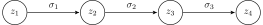
\includegraphics{neural1d.svg}

where

\begin{align*}
  z_2 = \sigma_1(z_1) = \sigma(a + b z_1)\\
  z_3 = \sigma_2(z_2) = \sigma(c + d z_2)\\
  z_4 = \sigma_3(z_3) = \sigma(e + f z_3),
\end{align*}
and $\sigma$ is the sigmoid function. This neural network has input $z_1$ 
and output $z_4$. Let $C$ be a function of the output $z_4$. For fixed
$z_1$, we consider $C$ as a function of $a, b, c, d, e, f$ via
$$
F\begin{pmatrix} a\\ b\\ c\\ d\\ e\\ f\end{pmatrix} =
C(\sigma_3(\sigma_2(\sigma_1(z_1)))).
$$
Backpropagation for training neural networks is using the
chain rule for computing the gradient
$$
\nabla F = \left( \pd{F}{a}, \pd{F}{b}, \pd{F}{c}, \pd{F}{d}, \pd{F}{e}, \pd{F}{f} \right).
$$

Explain how this is
done using the chain rule. Why is the method called backpropagation?

\begin{hideinbutton}{Hint}
  $$
  \pd{F}{z_3} = \pd{F}{z_4} \pd{z_4}{z_3}
  $$
  and
  $$
  \pd{F}{c} = \pd{F}{z_3} \pd{z_3}{c}
  $$
\end{hideinbutton}

\endshex





\section{Lagrange multipliers}\label{Lagrangemult}


The method of \url{Lagrange multipliers}{https://en.wikipedia.org/wiki/Lagrange_multiplier} is a super classical way of solving
optimization problems with non-linear (equality) constraints. We will only
consider the special case

  \begin{align}\label{lagrange}
    &\text{Maximize/Minimize} &f(x_1, \dots, x_n)\\
    &\text{with constraint}\\
    &&g (x_1, \dots, x_n) = 0,
  \end{align}

  where both $f:\RR^n\rightarrow \RR$ and $g:\RR^n\rightarrow \RR$ are
  differentiable functions.

  There is a very useful trick for attacking \eqref{lagrange}. One introduces an
  extra variable $\lambda$ (a Lagrange multiplier) and the Lagrangian function
  $L:\RR^{n+1}\rightarrow \RR$ given by
  $$
  L(x_1, \dots, x_n, \lambda) = f(x_1, \dots, x_n) + \lambda g(x_1, \dots, x_n).
  $$

  The main result is the following.

  \begin{theorem}[emph]\label{lagrmultthm}
    Suppose that $(z_1, \dots, z_n)$ is a local maximum/minimum for \eqref{lagrange}. Then there exists
    $\lambda\in \RR$, such that $(z_1, \dots, z_n, \lambda)$ is a critical point for $L$.
  \end{theorem}


  So to solve \eqref{lagrange} we simply (well, this is not always so simple) look for critical points for
  $L$. This amounts to solving the $n+1$ (non-linear) equations coming from $\nabla L = 0$ i.e.,
  \begin{align}
    g(x_1, \dots, x_n) &= 0\\
    \pd{f}{x_1}(x_1, \dots, x_n) + \lambda \pd{g}{x_1}(x_1, \dots, x_n) &= 0\\
                       &\vdots\\
    \pd{f}{x_n}(x_1, \dots, x_n) + \lambda \pd{g}{x_n}(x_1, \dots, x_n) &= 0         
  \end{align}

  For $n=2$ we can quickly give a sketch of the idea behind the proof. The (difficult) fact is that
  we may find a differentiable function $x(t)$ in one variable $t$, such that
  $$
  g(t, x(t)) = 0
  $$
  and the local minimum has the form $v_0 = (t_0, x(t_0))$.
  
  Once we have this, the chain rule does its magic. We consider the one variable functions
  \begin{align}
    F(t) &= f(t, x(t))\\
    G(t) &= g(t, x(t))
  \end{align}
  For both of these we have $F'(t_0) = G'(t_0) = 0$ (why?). The
  chain rule now gives a non-zero vector orthogonal to $\nabla f(v_0)$ and $\nabla g(v_0)$. This is
  only possible if they are parallel as vectors i. e. , there exists $\lambda$, such that
  $$
  \nabla f (v_0) = \lambda \nabla g (v_0).
  $$

  \begin{example}\label{minlagr}
    Consider the minimization problem
\begin{align*}
    &\text{Minimize} &x+y\\
    &\text{with constraint}\\
    &&x^2 + y^2 = 1.
  \end{align*}
  First of all, why does this problem have a solution at all? We write
  the non-linear equations
  \begin{align*}
    1 + 2 x\lambda &= 0\\
    1 + 2 y\lambda &= 0\\
    x^2 + y^2 - 1&= 0
  \end{align*}
  up coming from the critical points of the Langrange function. Now we know that
  these can be solved and that amongst our solutions there is a minimum!
  \end{example}


  \beginshex
  Use Theorem \ref{lagrmultthm} to
maximize $x^2 + y^2$ subject to $x^2 + x y + y^2 = 4$. 

\begin{hideinbutton}{Hint}
Here you end up with the system
\begin{align*}
(2\lambda + 2) x  + \lambda y &= 0\\
\lambda x + (2\lambda + 2) y &= 0
\end{align*}
of linear equations in $x$ and $y$, where you
regard $\lambda$ as a constant. Use Gaussian
elimination to solve this system in order to
derive a (nice) quadratic equation in $\lambda$ coming from
$$
-\frac{\lambda}{2\lambda +2} \lambda y + (2 \lambda + 2) y = 0
$$
and $y\neq 0$.
\end{hideinbutton}


Consider the subset
$C = \{(x, y)\in \RR^2\mid x^2 + x y + y^2 = 4\}$. Why is $C$ a closed subset?
Why is $C$ bounded? 

\begin{hideinbutton}{Hint}
To prove that $C$ is bounded you can keep $y$ fixed in 
\begin{equation}\label{ellipsis4}
x^2 + y x + y^2 - 4 = 0
\end{equation}
and solve for $x$. A last resort is using the plot in Sage in the Hint button below, but that
does not give any real insight unless you explain how Sage makes the plot from
the equation \eqref{ellipsis4}.
\end{hideinbutton}

How does this relate to Theorem \ref{thmcontcomp}?

Does the optimization
problem have a geometric interpretation?

\begin{hideinbutton}{Hint}
  \begin{sage}
x, y = var('x, y')
implicit_plot(x^2 + x*y + y^2 - 4, (x, -3, 3), (y, -3, 3))
  \end{sage}
\end{hideinbutton}

\endshex


\beginshex
  A rectangular box has side lengths $x$, $y$ and $z$. What is its
  maximal volume when we assume that $(x, y, z)$ lies on the plane
  \begin{equation*}
    \frac{x}{a} + \frac{y}{b} + \frac{z}{c} = 1
  \end{equation*}
  for $a, b, c > 0$.
\endshex


\beginshex\label{boxlagr}
  A company is planning to produce a box with volume
  $2$ $m^3$. For design reasons it needs different
  materials for the sides, top and bottom. The cost of the materials
  per square meter is $1$ dollar for the sides, $1.5$ dollars for the
  bottom and the top. Find the measurements of the box minimizing the
  production costs.
\endshex


\beginshex
  \begin{align*}
    &\text{Maximize} &- p_1 \log_2(p_1) - \cdots - p_n \log_2(p_n)\\
    &\text{with constraint}\\
    &&p_1 + \cdots + p_n = 1.
  \end{align*}

\endshex


\section{The interior and the boundary of a subset}

Suppose that $C\subseteq \RR^n$ is a compact subset and $f:\RR^n\rightarrow \RR$ is a
continuous function. Recall (see Theorem \ref{thmcontcomp}) that the
optimization problem
  \begin{align*}
    &\text{Optimize} &f(x)\\
    &\text{with constraint}\\
    &&x\in C
  \end{align*}
  always has a solution. To solve such an optimization problem, it often
  pays to decompose $C$ as
  $$
  C = \partial C \cup C^o,
  $$
  where $\partial C$ is the boundary of $C$ and $C^o$ the interior of $C$.

  The boundary of $C$ is the set of points in $C$, which are limits of both
  convergent sequences with elements not in $C$ and convergent sequences with elements in $C$.
Informally these are points in $C$,
  that can be approximated (arbitrarily well) both from outside $C$ and from inside $C$.

\beginshex
What are the boundary points of $(0, 1)\subseteq \RR$?
\endshex  


  The interior of $C$ is the set of points in $C$, which are
  not limits of convergent sequences with elements not in $C$. Informally these are points in $C$,
  that cannot be approximated (arbitrarily well) from outside $C$.

  \beginshex
  Compute the boundary and the interior of the subset $\{1, 2, 3\}\subseteq \RR$.
  
  What is the interior and the boundary of the subset $[0, 1] \subseteq \RR$?
  \endshex

  If $x_0$ is an element of $C^o$, then there exists an open subset
  $U\subseteq C$, such that $x_0\in U$. Therefore the following proposition holds, when you take Proposition \ref{locopt} into account.

  \begin{proposition}[emph]\label{propint}
    Consider an optimization problem
  \begin{align}\label{addopt}
    &\text{Optimize} &f(x)\\
    &\text{with constraint}\\
    &&x\in C,
  \end{align}
  where $C\subseteq \RR^n$ is a subset, $f:\RR^n\rightarrow \RR$ a
  differentiable function and $x_0$ an optimal solution to \eqref{addopt}. If $x_0\in C^o$, then $x_0$ is a critical point of $f$.
\end{proposition}


Basically, to solve an optimization problem like \eqref{addopt} one needs to
consider the boundary and interior as separate cases. For points on
the boundary we cannot use the critical point test in Proposition \ref{locopt}.
This test only applies to the interior points. Usually the boundary cases
are of smaller dimension and easier to handle as illustrated in the example below.



\begin{example}
    Consider the minimization  problem
\begin{align*}
    &\text{Minimize} &x+y\\
    &\text{with constraint}\\
    &&x^2 + y^2 = 1.
  \end{align*}
  from Example \ref{minlagr}. Let us modify it to
\begin{align}\label{minmodif}
    &\text{Minimize} &x+y\\
    &\text{with constraint}\\
    &&(x, y)\in C,
\end{align}
where
$$
C=\{(x, y)\in \RR^2 \mid x^2 + y^2\leq  1\}.
$$
We are now minimizing not only over the unit circle, but
the whole unit disk. Here
$$
\partial C = \{(x, y)\in \RR^2 \mid x^2 + y^2 = 1\}\quad
\text{and}\quad
C^o = \{(x, y)\in \RR^2 \mid x^2 + y^2 < 1\}.
$$
Proposition \ref{propint} guides us first to look for
optimal points in $C^o$. Here we use Proposition \ref{locopt} to
show that there can be no optimal points in $C^o$, because
the gradient of the function $f(x, y) = x + y$ is
$$
\nabla f = (1, 1).
$$
Therefore the boundary needs to be analyzed and the usual technique
(as was implicit in Lagrange multipliers) is to find
a parametrization for the points $(x, y)$ satisfying
$x^2 + y^2 = 1$. There are two of those (one for the upper unit circle and one for the lower unit circle):
\begin{align*}
  &\left(t, \sqrt{1 - t^2}\right)\\
  &\left(t, -\sqrt{1 - t^2}\right),
\end{align*}
where $t\in [-1, 1]$.
This means that the optimization problem for the boundary $C^o$ turns into the two
simpler optimization problems of minimizing
$$
t + \sqrt{1 - t^2}\qquad \text{and}\qquad t - \sqrt{1 - t^2}
$$
subject to $t\in [-1, 1]$. These can as one variable optimization problems be solved the usual way.
\end{example}


The
exercises below are taken from the Calculus book.


\beginshex\label{calcopt1}
Solve the two optimization problems
  \begin{align*}
    &\text{Maximize/Minimize} &x^2 - 2 x y + 2 y\\
    &\text{with constraint}\\
    &&(x, y)\in C,
  \end{align*}
  where $C = \{(x, y)\in \RR^2 \mid 0\leq x \leq 3, 0\leq y \leq 2\}$. But first give a
  reason as to why they both are solvable.
  
  \begin{hideinbutton}{Hint}
    First find $\partial C$ and $C^o$. Then try with Proposition \ref{propint}
    supposing that a maximal point really is to be found in $C^o$ and not
    on $\partial C$.
  \end{hideinbutton}
\endshex


\beginshex\label{calcopt2}
Solve the two optimization problems
  \begin{align*}
    &\text{Maximize/Minimize} &1 + 4 x - 5 y\\
    &\text{with constraint}\\
    &&(x, y)\in C,
  \end{align*}
  where $C = \{(x, y)\in \RR^2 \mid 0\leq x, 0\leq y, 3 x + 2 y \leq 6\}$. But first give a
  reason as to why they both are solvable.
\endshex


\beginshex\label{calcopt3}
Solve the two optimization problems
  \begin{align*}
    &\text{Maximize/Minimize} &3 + x y - x - 2 y\\
    &\text{with constraint}\\
    &&(x, y)\in C,
  \end{align*}
  where $C$ is the triangle with vertices in $(1, 0), (5, 0)$ and $(1, 4)$. But first give a
  reason as to why they both are solvable.
\endshex

\beginshex
Use Proposition \ref{propint} to give all the minute details in applying
Theorem \ref{lagrmultthm} to solve Exercise \ref{boxlagr}.
\endshex
  
  
\end{document}